\section{Procedure}
\label{sec:Durchführung}

The setup for measuring the heat capacity is shown in \autoref{fig:aufbau}.
In the middle of the recipient is a copper cylinder with a heating coil around it which are both in a dewar vessel for thermal insulation.
The probe is inside of the cylinder.
Also there are two resistors to measure the temperature of the cylinder and the probe.
\begin{figure}
    \centering
    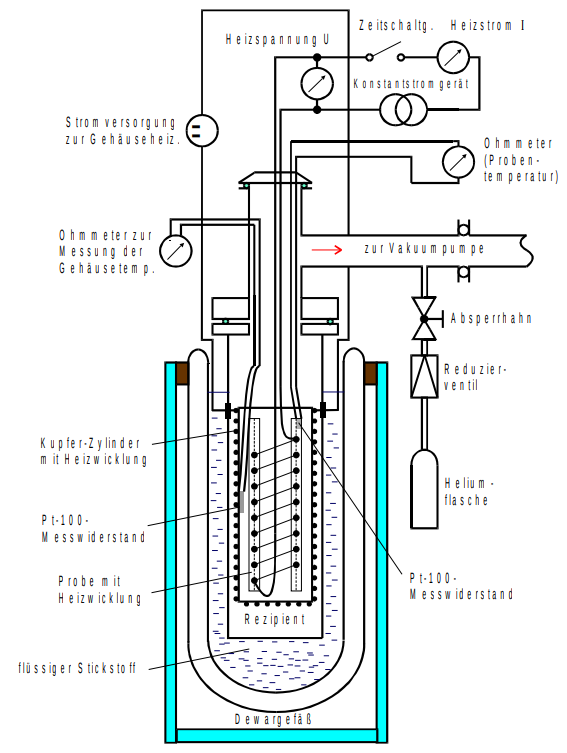
\includegraphics[width=0.8\textwidth]{content/plots/aufbau.png}
    \caption{Schematic view of the used structure to measure the heat capacity \cite{V47}.}
    \label{fig:aufbau}
\end{figure}
Before starting the experiment we need to create a vacuum inside of the recipient and fill it with helium.
The dewar vessel gets filled with fluid nitrogen to cool the probe and cylinder to around $\qty{80}{\kelvin}$.
After the cooling process the vacuum pump is turned on again to lower the pressure inside.
But before heating the copper, the helium gets extracted from the recipient.
The actual experiment starts when the heating coil starts heating the probe.
To minimize energy loss, the cylinder is kept at the same temperature with its own heating coil.
In order to be able to determine the supplied heat energy, the voltage, the current and the heating time are noted down after the temperature has risen by about $\qty{10}{\kelvin}$.
As soon as the temperature reaches about $\qty{300}{\kelvin}$, the measurement is to be stopped.